\section{Betriebssysteme - Grundlagen}

\question{Welche zwei Hauptaufgaben hat ein Betriebssytem?}
\begin{answer}
    \begin{itemize}
    \item \crucial{Abstraktion von Ger"ateeigenschaften}
        \begin{itemize}
            \item Geräteunabh"angige Schnittstelle zu den Anwendungen 
            \item Geräteüberwachung und -steuerung
        \end{itemize}
    
    \item \crucial{Unterst"utzung des Mehrbenutzerbetriebs}
        \begin{itemize}
            \item Betriebsmittelverwaltung
            \item Zuteilungsstrategien
            \item Kostenabrechnung
            \item Schutz
        \end{itemize}
    \end{itemize}
\end{answer}

\question{Was ist ein Prozess?}
\begin{answer}
Ein \crucial{Programm in Ausf"uhrung}.
\end{answer}

\question{Was sind Dateien?}
\begin{answer}
Dateien sind \crucial{langlebige, "uber eindeutige Namen (Pfade) identifizierbare Datenobjekte}. Prozesse können auf sie zugreifen und sie modifizieren (wenn die nötige Berechtigung gegeben ist). Für UNIX stellt der Inhalt lediglich eine Bytefolge dar (beliebige interne Struktur).
\end{answer}

\question{Welche Arten von Dateien gibt es?}
\begin{answer}

\begin{itemize}
\item Normale Dateien (plain files)
\item Verzeichnisse
\item Symbolische Links
\item Geräte-Dateien
	\begin{itemize}
	\item Blockorientierte Gerätedateien
	\item Zeichenorientierte Gerätedateien
	\end{itemize}
\item Sockets~(\ref{netzwerke:sockets}) und Named Pipes~(\ref{netzwerke:named-pipe})
\end{itemize}

\end{answer}

\question{Wie ist ein UNIX-Dateisystem strukturiert? Wie können Dateien darin (eindeutig) aufgefunden
werden?}
\begin{answer}
Ein UNIX-Dateisystem ist eine \crucial{hierachisch organisierte} Verzeichniss-Struktur. Ganz oben steht \crucial{ die Wurzel} (root). In Vezeichnissen können Dateien abgelegt werden. Vollständige Dateinamen (absoluter Pfad) sind (eindeutige) \crucial{Pfadnamen} von der Wurzel abwärts. Relative Pfade sind ebenfalls möglich.
\end{answer}

\question{Was ist ein \textit{symbolic link} (symbolischer Link)?}
\begin{answer}
Ein \textit{ symbolic link} ist ein \crucial{Verweis auf eine Datei oder auf ein Verzeichnis} (, die nicht notwendigerweise existieren müssen). Es ist also lediglich eine Referenz auf die Zieldatei bzw. das Zielverzeichnis (d.h. ein weiterer Pfad zu einer Datei). Ein Löschen oder Verschieben der eigentlichen Datei oder das Verweisen auf eine nicht existierende Datei führen üblicherweise dazu, dass die Referenz „ins Leere“ weist \crucial{(dangling link)}.

\question{Was ist ein \textit{hard link}?}
\paragraph*{}
Ein \crucial{Hardlink} ist im Grunde genommen ein \crucial{weiterer, regul"arer Name der Datei} (Zwei Namen für die selbe Datei). Wird also die Datei unter ihrem ursprünglichen Namen gelöscht, ist sie unter ihrem zweiten Namen immer noch vorhanden. Erst wenn alle "Namen" gelöscht sind ist die Datei nicht mehr zugreifbar. Intern wird dies durch Reference-Counting erreicht. Hardlinks \crucial{k"onnen nicht auf Verzeichnisse gelegt werden} (Vermeidung unkontrollierte Schleifen).
\end{answer}

\question{Ist das UNIX-Dateisystem wirklich ein Baum? Begründung.}
\begin{answer}
Ein UNIX-Dateisystem entspricht eher einem \crucial{gerichteten Graphen} als einem Baum. Verzeichnisse und Dateien sind zwar hirarchisch organisiert, aber Möglichkeit von \crucial{Hardlinks}, d.h. das mehrfache Vorhandensein in der Dateistruktur einer physikalisch nur einfach vorhanden Datei stört das Bild eines Baumes. In einem Baum werden die Knoten benannt, unter UNIX werden Pfadnamen benutzt.
\end{answer}

\question{Welche Zugriffsrechte kann man auf eine UNIX-Datei haben? Welche Dateiattribute steuern dies, und wie?}
\begin{answer}
Die Zugriffsrechte sind \crucial{Lesen}, \crucial{Schreiben} und \crucial{Ausf"uhren}.
Es können unterschiedliche Rechte für den \crucial{Besitzer} (user) einer Datei, die \crucial{Gruppe} (group) und den \crucial{Rest der Welt} (others) festgelegt werden. Zusätzlich gibt es noch die erweiterten Rechte \crucial{Setuid}, \crucial{Setgid} und das \crucial{Sticky Bit.}\footnote{http://de.wikipedia.org/wiki/Unix-Dateirechte\#Sonderrechte.2Ferweiterte\_Rechte}

\subsection*{Detaillierte Auflistung der Zugriffsrechte:}
{\tiny\bfseries
\renewcommand{\arraystretch}{1.5}
	\begin{center}
	  \begin{tabular}{ | p{1.3cm} ||
	  >{\color{blue}\centering\arraybackslash}m{1.5cm} |
	  >{\color{blue}\centering\arraybackslash}m{1.5cm} |
	  >{\color{blue}\centering\arraybackslash}m{1.5cm} ||
	  >{\color{dkgreen}\centering\arraybackslash}m{1.2cm} |
	  >{\color{dkgreen}\centering\arraybackslash}m{1.2cm} |
	  >{\color{dkgreen}\centering\arraybackslash}m{1.2cm} ||
	  >{\color{dkgreen}\centering\arraybackslash}m{0.8cm} |
	  >{\color{dkgreen}\centering\arraybackslash}m{0.8cm} |}
	    \hline
	     
	     &  \multicolumn{3}{c||}{Erweiterte Rechte} & \multicolumn{3}{c||}{User (Owner)} & \textcolor{black}{Group} & \textcolor{black}{Others} \\ \hline
	     
	     & SUID & SGID & Sticky & r & w & x & r w x & r w x  \\ \hline
	    
	    \textbf{Plain file} & \uline{Ausf"uhren:} Benutzer vs. \uline{Besitzer der Datei} & \uline{Ausf"uhren:} Benutzer vs. \uline{Dateigruppe} & (Bleibt im Swap Space kleben) & Lesen & Schreiben & Ausführen & (dito) & (dito)  \\ \hline
	    
	    \textbf{Directory} &  & Dateien darin erhalten Gruppe der Dir & Nur eigene Dateien in Dir löschbar (bsp.: /tmp) & Einträge lesen & Einträge (indirekt) ändern & Auf Dateien darin zugreifen & (dito) & (dito)  \\ \hline
	  \end{tabular}
	\end{center}
}
\end{answer}

\question{Welche Vorteile bietet es, auf Terminals in UNIX wie auf Dateien zuzugreifen? Was versteht man unter Ein-/Ausgabeumlenkung?}
\begin{answer}
Da unter \textbf{UNIX} der Zugriff auf Geräte im allgemeinen (d.h. auch auf Terminals) als Zugriff auf eine Dateien abgebildet sind, bietet dies den Vorteil der \crucial{einheitlichen Schnittstelle und Handhabung}. Der Benutzer
kann auf das Terminal zugreifen wie auf eine Datei auch und muss sich daher nicht mit den konkreten Geräteeigenschaften auseinandersetzen. \\
Es gibt \crucial{Standardein- und Standardausgaben von Prozessen}. Will der Benutzer andere Ein- bzw. Ausgabemöglichkeiten nutzen, kann er Ein- und Ausgaben umlenken. Beispielsweise können die Fehlermeldungen in eine Datei umgelenkt werden.

%% Bash script
\lstset{language=bash,caption={Ein-/Ausgabeumlenkung}}
\begin{lstlisting}
user $ echo -e "#\!/bin/bash\necho Hello world" > /tmp/bla # (1)
user $ bash < /tmp/bla # (2)
Helloworld
\end{lstlisting}

\begin{enumerate}
\item Die Ausgabe des Befehls \texttt{echo} wird in eine Datei \texttt{/tmp/bla} geschrieben, und somit eine Ausgabeumlenkung getätigt.

\item Unter (2) liest die neu erzeugte shell von der soeben erstellten Datei \texttt{/tmp/bla} anstelle des Terminal, was einer Eingabeumlenkung entspricht.
\end{enumerate}

\end{answer}

\question{Welche Aufgabe hat ein Kommando-Interpreter (z.B. in UNIX die Shell)?}
\begin{answer}
Ein Kommando-Interpreter stellt dem Benutzer eine einfache (und zugleich mächtige) Schnittstelle zum Betriebssystem \crucial({Benutzungsschnittstelle}) zur Verfügung. Damit lassen sich Aufträge an das Betriebssystem absetzen. Die Shell ist ebenfalls ein Prozess.
\end{answer}

\question{Was machst Du, wenn Dir die genaue Semantik eines Unix-Kommandos entfallen ist?}
\begin{answer}
Zunächst die Hilfe (mit dem \crucial{Kommandozeilenswitch --help}), und wenn erforderliche die \crucial{Man-} oder \crucial{Infopages} zur Rate ziehen:
%% Bash script
\lstset{language=bash,caption={Hilfe zu einem Kommando am Beispiel von \texttt{mkdir}}}
\begin{lstlisting}
user $ mkdir --help
user $ man mkdir
user $ info mkdir
\end{lstlisting}
\end{answer}

\begin{multilinequestion}[\texttt{bla} sei ein ausführbares Programm. Was ist der Unterschied zwischen dem Aufruf]

%% Bash script
\lstset{caption={}}
\begin{lstlisting}
bla
\end{lstlisting}

und dem Aufruf

%% Bash script
\lstset{caption={}}
\begin{lstlisting}
bla &
\end{lstlisting}

in der Shell? Welche Auswirkungen hat dies, wenn \texttt{bla} von \textbf{Standard Input} liest bzw. auf \textbf{Standard Output} schreibt?
\end{multilinequestion}

\begin{answer}
\texttt{bla} wird im \crucial{Vordergrund} ausgeführt und beansprucht das Terminal (=Tastatur) für sich. Weitere Shell-Eingaben sind daher erst möglich, nachdem \texttt{bla} terminiert.

\paragraph{}
Hängt man einem Befehl ein \& an, so wird dieser im \crucial{Hintergrund} ausgeführt (Hintergrundprozess). Er gibt damit die Kontrolle über das Terminal auf, so dass dieses für neue Prozesse verwendet werden kann. Dieser \crucial{kann} dann zwar auf \texttt{stdout} \crucial{schreiben}, wird aber sofort in den Zustand \crucial{suspended} versetzt , \crucial{wenn er versucht von der Standardeingabe (\textit{stdin}) zu lesen}.
\end{answer}

\begin{multilinequestion}[Prozessbäume: Gegeben sei der folgende Prozessbaum:]

\begin{figure}[H]
  \caption{Prozessbaum}
  \centering
    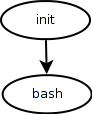
\includegraphics[scale=0.70]{images/process-tree01}
\end{figure}

Wie ändert er sich nach Eingeben der folgenden Kommandofolge im Shell?

%% Bash script
\lstset{language=bash,caption={Eingegebene Befehle}}
\begin{lstlisting}
sleep 1000 &
emacs &
bash
date
\end{lstlisting}

\end{multilinequestion}

\begin{answer}
Der Prozessbaum sieht nach Eingabe der obigen Befehle folgendermaßen aus:
\begin{figure}[H]
  \caption{Prozessbaum nach den Eingaben}
  \centering
    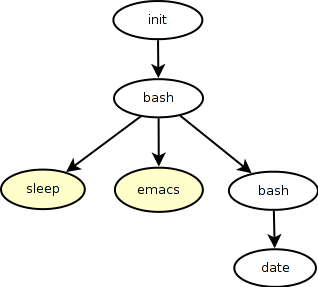
\includegraphics[scale=0.70]{images/process-tree02}
\end{figure}
\texttt{sleep} und \texttt{emacs} laufen dabei als Hintergrundprozesse.
\end{answer}


\question{Nenne drei Beispiele für Informationen, die der Betriebsystemkern über einen Prozess wissen muss.}
\begin{answer}
\begin{itemize}
\item \crucial{Prozess ID}
\item \crucial{Parent-Prozess ID}
\item \crucial{Zustand des Prozesses}
\end{itemize}

\end{answer}

\question{Was ist eine Pipe?}
\begin{answer}
Eine Pipe ist die \crucial{Umlenkung} eines \crucial{unidirektionalen sequentiellen Bitstroms} von der \crucial{Standardausgabe} eines Prozesses auf die \crucial{Standardeingabe} eines Prozesses.
\end{answer}

\question{Wie macht man ein soeben editiertes Shell-File ausführbar?}
\begin{answer}
\crucial{Setzen des Ausf"uhrbar-Bits} (executable bit) (x). \\

%% Bash script
\lstset{language=bash,caption={Setzen des \textbf{executable bit} für ein Shellskript \textit{shellfile.sh}}}
\begin{lstlisting}
chmod +x shellfile.sh
\end{lstlisting}

\end{answer}

\question{In welche Bereiche (Segmente) ist der virtuelle Adressraum eines Programmes in Ausführung unter UNIX unterteilt, und welche Eigenschaften kennzeichnen sie?}
\begin{answer}
Der virtuelle Adressraum ist in \crucial{Text}, \crucial{Data} und \crucial{Stack} unterteilt. Im Text-Teil befindet siche
der eigentliche Programmcode, im Data-Teil die Daten und auf dem Stack alle temparären
Daten (z.B. Variablen).
\end{answer}

\question{Wozu wird der Stack verwendet?}
\begin{answer}
Auf einem Stack werden die \crucial{innerhalb von Funktionsaufrufen tempor"ar anfallenden Daten eines Prozesses} abgelegt. Das umfasst unter anderem die Rücksprung-Addresse, die an die Funktion übergebenen Argumente und lokale Variablen.
\end{answer}

\question{Welchem Zweck dienen Bibliotheken (Libraries)?}
\begin{answer}
Bibliotheken \crucial{stellen Funktionen zur Verf"ugung}. Durch das Vorhandensein von Bibliotheken muss ein Programmierer nicht von Grund auf alle Funktionen neu schreiben.

\paragraph{}
Eine Programmbibliothek bezeichnet in der Programmierung eine \crucial{Sammlung von Softwaremodulen}, die Lösungswege für thematisch zusammengehörende Problemstellungen anbieten. Bibliotheken sind im Unterschied zu Programmen keine eigenständig lauffähigen Einheiten, sondern Hilfsmodule, die von Programmen angefordert werden.\footnote{http://de.wikipedia.org/wiki/Programmbibliothek}

\end{answer}

\question{Welche Aufgabe erfüllt ein Linker?}
\begin{answer}
Ein Linker oder Binder verbindet einzelne Programmmodule zu einem ausführbaren Programm. Im Zuge dessen werden die Symbole in den Objectfiles aufgelöst. Man unterscheidet zwischen statisches und dynamisches Linken. Man unterscheidet dabei zwischen \crucial{statisches und dynamisches Linken}.

\paragraph*{Statisches Linken:}
Die Symbole schon während des Zusammenstellens der Programmdatei aufgelöst

\paragraph*{Dynamisches Linken:}
Das Auflösen der Symbole erfolgt erst bei der tatsächlichen Ausführung des Programms.
\end{answer}

\question{Wozu wird beim Assemblieren eine Symboltabelle angelegt?}
\begin{answer}
Zum Auflösen von Verweisen.
\end{answer}

\question{Welchen Vorteil hat es, Bibliotheken mit \textit{Position Independent Code} zu versehen?}
\begin{answer}
Position-independent Code (PIC, engl. für positionsunabhängiger Code) ist \crucial{Maschinencode, der ausgef"uhrt werden kann, unabh"angig davon, an welcher absoluten Adresse im Hauptspeicher er sich befindet}. PIC wird üblicherweise für dynamische Bibliotheken verwendet, damit diese für jedes Programm an eine Speicherposition geladen werden können, wo sie sich nicht mit anderen Objekten dieses Programms überlappen.\footnote{http://de.wikipedia.org/wiki/Position-Independent\_Code} 
\end{answer}

\question{Durch welche "Qualitätsmerkmale" sollten Betriebssysteme gekennzeichnet sein? Nenne Beispiele für konkurrierende Anforderungen.}
\begin{answer}
\crucial{Effizienz, Kosten, Bedienbarkeit, Zuverl"assigkeit, Verf"ugbarkeit, Sicherheit, Wartbarkeit.
Der Kostenpunkt kann mit jeder anderen Anforderung konkurrieren.} Je besser ein Aspekt werden soll, desto mehr Zeit und Entwicklungsarbeit, sprich Geld muss in diesen Aspekt investiert werden. Am Beispiel Windows lässt sich wunderbar erkennen, wie \crucial{Bedienbarkeit und Zuverl"assigkeit im Widerspruch} zueinander stehen können. Die Sicherheit eines OS's lässt sich oft auch nicht mit einer ausgereiften Bedienbarkeit vereinbaren, oder umgekehrt, siehe Win vs. Linux.
\end{answer}

\question{Worin unterscheidet sich der Kernel-Mode vom User-Mode (in UNIX)? Warum wird diese Unterscheidung getroffen?}
\begin{answer}
\crucial{Kernel und Useradressraum sind aus Sicherheitsgr"unden getrennt. Im User-Mode gibt es keinen direkten Zugriff auf die Hardware.} Das hat auch seinen Sinn, da diese Zugriffe kontrolliert erfolgen sollen, damit das System sicher und zuverlässig bleibt.
\end{answer}

\question{Was passiert etwa bei einem System-Aufruf? (Reihenfolge der Arbeitsschritte.)}
\begin{answer}
\crucial{Es erfolgt ein Trap, darauf wird der Zustand des Systems gesichert, dann erfolgt der Sprung in den Kernel-Mode, in dem der eigentliche Hardware-Zugriff erfolgt. Daraufhin gibt es eine R"uckmeldung und einen R"ucksprung zum Prozess, wo dann auch der Kontext wieder hergestellt wird.}
\end{answer}

\question{Was ist ein Interrupt? Nenne Beispiele für mögliche Interrupt-Quellen. Warum werden sie unterschiedlich priorisiert? Wie wird ein Interrupt in etwa behandelt?}
\begin{answer}
Ein Interrupt ist eine externe Unterbrechung eines Prozesses. Eine Quelle kann z. Bsp. die
Hardware sein. Hardwareinterrupts haben generell eine höhere Priorität als Softwareinterrupts.
Beim Clock-Tic ist die Quelle eben die Hardware, und der Prozess hat eine sehr hohe
Priorität, da ansonsten die System-Uhr nicht mehr genau laufen würde, was sich fatal auf
andere Programme auswirken kann, die sich nach dieser Uhr zu richten haben.
Beispiele für einen Softwareinterrupt wären SIGKILL oder SIGSTOP.
\end{answer}

\question{Was ist ein Trap? Nenne Beispiele. Inwiefern unterscheiden sich Traps von Interrupts?}
\begin{answer}
Ein Trap ist ein interne Unterbrechung eines Programms in Ausführung, die vom System
kommt. Beim Trap wird in den Kernel-Mode gewechselt, da es ja ein Systemaufruf ist.
Die Regelung erfolgt durch den Trap-Handler, der bei Bedarf dann auch Signale senden
kann. Division durch 0 wäre ein solches Beispiel. Es wird ein Trap ausgelöst, der durch den
Trap-Handler gejagt wird, welcher wiederum das Signal sigfpe lossendet (SignalFloating-
PointError). Die Folge ist, wie bei vielen anderen Signalen auch, dass der Prozess terminert
oder gekillt wird.
\end{answer}

\question{Was ist ein Signal? Nenne Beispiele für mögliche Signalquellen. Wie kann ein Prozess auf ein Signal reagieren?}
\begin{answer}
Signale dienen der Meldung (von Ausnahmezust"anden) an einen Prozess. Sowohl der Benutzer als auch Prozesse können Signale an Prozesse senden. Beispiele für Signale sind u.a. Stop (SIGINT), Kill (SIGKILL), Terminate und (SIGTERM). Der Traphandler ist oft eine Signalquelle.
\end{answer}

\question{Beschreibe kurz einige Zustände, in denen sich ein (UNIX-)Prozess befinden kann.}
\begin{answer}
\subsection*{Einfaches Modell:}
\begin{itemize}
\item Ready
\item Run
\item Sleep
\item Zombie
\end{itemize}


\subsection*{Erweitertes Modell:}

\begin{description}
\item[dead]\hfill \\ Der Prozess wurde beendet, er belegt jedoch noch Speicherplatz.

\item[ready]\hfill \\ Der Prozess wartet auf Zuteilung der CPU (Zeitschlitz). Gibt es den Ready-Zustand, so befinden sich höchstens so viele Prozesse im Zustand running, wie CPUs vorhanden sind.

\item[running]\hfill \\ Entweder genau der Prozess, der gerade bearbeitet wird, oder alle Prozesse, die momentan Rechenarbeit verrichten können.

\item[sleep]\hfill \\ Der Prozess wurde auf eigenen Wunsch zurückgestellt. Er kann Signale entgegennehmen, wie z. B. Timer, oder Ergebnisse von Kindprozessen.

\item[trace]\hfill \\ Der Prozess wurde von außen angehalten, üblicherweise durch einen Debugger.

\item[wait]\hfill \\ Der Prozess wartet auf ein Ereignis, üblicherweise eine Benutzereingabe.

\item[uninterruptible sleep]\hfill \\ Der Prozess wartet auf ein Ereignis, üblicherweise Hardware. Tritt dieses Ereignis ein, ohne dass der anfragende Prozess es entgegennimmt, so kann das System instabil werden.

\item[zombie]\hfill \\ Der Prozess wurde beendet und aus dem Arbeitsspeicher gelöscht, aber noch nicht aus der Prozessliste entfernt.
\end{description}

\end{answer}

\question{Nenne einige Randbedingungen, auf die man beim Entwurf eines Schedulers achten sollte. Wie sollten rechenintensive bzw. Ein-/Ausgabe-intensive Prozesse dabei behandelt werden?}
\begin{answer}
Ein Scheduler soll schlank (effizient) und fair sein, d. h. der Rechenaufwand der Prozessverwaltung
darf nicht so gross werden, dass die Effizienz darunter leidet, und jeder Prozess soll
gerechterweise auch drankommen. Auch die Zeitscheiben sollen eine angemessene Grösse
haben.
\end{answer}

\question{Wie könnte man mit Hilfe eines Round-Robin-Schedulers Prozess-Prioritäten "simulieren"?}
\begin{answer}
Man könnte die Anzahl der Durchläufe für die Prozesse mit einer hohen Priorität erhöhen,
so dass diese in einem Durchlauf mehrere Male dran kommen, oder man gibt den wichtigen
Prozessen grössere Zeitscheiben, um ihnen mehr CPU-Zeit zukommen zu lassen.
\end{answer}

\question{Warum bestehen die \textit{Sleep}- und die \textit{Run-Queue} in UNIX nicht aus jeweils einer einzigen Warteschlange? Wie sind sie stattdessen organisiert?}
\begin{answer}
Sleep-Queue und Run-Queue bestehen aus jeweils einem Array. Jede Priorität hat darin
eine eigene Liste, das Handling zwischen den Queues ist abhängig von der Priorität. Diese
Aufteilung besteht, da sonst immer alles durchsucht werden müsste.
\end{answer}

\question{Warum werden die Zustandsinformationen eines UNIX-Prozesses teilweise in der \textit{Proc-Struktur} und teilweise in der \textit{User-Struktur} abgelegt? Nenne jeweils drei charakteristische Beispiele für Angaben darin.}
\begin{answer}
Die in der Proc-Struktur abgelegten Zustandsinformationen sind für alle Prozesse verfügbar,
die in der User-Struktur abgelegten sind nur für den laufenden Prozess verfügbar.
Beispiele für Angaben in der Proc-Struktur:
Signale, die zur Verarbeitung anstehen
Prozesszustände
Scheduling
Beispiele für Angaben in der User-Struktur:
Zugriffsrechte
Aktuelles Verzeichnis
Geöffnete Dateien.
\end{answer}

\question{Skizziere kurz die Prozesserzeugung in UNIX. Welche Rolle spielen die Systemaufrufe fork() und exec() dabei? Wie unterscheiden sich Vater- und Kindprozess voneinander?}
\begin{answer}
Der Prozess Nummer Eins (init) wird ,,von Hand'' beim Systemstart erzeugt (standardmäßig \texttt{/sbin/init}, andere Pfade können dem Kernel im Boot-Loader als Parameter übergeben werden).
Andere Prozesse werden bei Bedarf als Kindprozesse mit fork() (oft als Kind-Prozesse
der Shell) erzeugt. So entsteht eine Hierachie von Prozessen. Der Kindprozess erhält eine
neue Prozess-ID, ist aber zunächst eine Kopie des Vaters, d.h. der ,,gleiche'' Adressraum
mit gleicher Aufteilung (d.h., gleiche Segmente) von Text, Data und Stack. Normalerweise soll das Kind ein anderes
Programm ausführen. Dieses wird mit exec() gestartet. Damit wird dann auch der
Adressraum ausgetauscht.
\end{answer}

\question{Wie erfährt ein UNIX-Prozess, ob ein Kindprozess terminiert ist? Wozu gibt es in UNIX den Prozesszustand SZOMB (,,Zombie'')?}
\begin{answer}
Das Kind meldet bei der Termination das Signal SIGCHLD an den Vater, dieser behnadelt
durch den Aufruf wait() den Kindprozess und der Kindprozess terminiert
oder der Vater ignoriert das Signal. In diesem Fall wird das Kind zum Zombie. Der Zombie
wird dann entweder später vom Vater behandelt oder (je nach UNIX-Variante) durch das
Betriebssystem. Z.B. kann der INIT-Prozess die Proc-Struktur wieder freigeben.
\end{answer}

\question{Wie werden mehrere Prozesse in einer Einprozessormaschine verwaltet?}
\begin{answer}
In einer Einprozessormaschine kann zu jedem Zeitpunkt nur ein Prozess in Ausführung sein.
Damit alle Programme einmal an die Reihe kommen und ausgeführt werden, gibt es den Scheduler.
Dieser ,,simuliert'' auf Einprozessormaschinen Parallelität, indem jeder Prozess nur für
einen begrenzten Zeitraum (,,Zeitfenster'') ausgeführt wird.

Es gibt innerhalb des Kernels zwei Warteschlangen: die Run- und die Sleep-Queue.
Letztere kommt zum Tragen, wenn ein Prozess sich schlafenlegt (zum Beispiel mit \texttt{sleep()}).
In diesem Fall wäre es unsinnig, den Prozess weiter auszuführen. Stattdessen findet ein Kontextwechsel
statt und ein anderer Prozess wird ausgeführt. Für letzteres existiert die Run-Queue. In dieser befinden
sich alle fortzuführenden Prozesse.

Für die Verwaltung der Warteschlangen gibt es unterschiedliche Strategien: FIFO und Shortest Job Next.
Bei ersterem werden die Prozesse nach und nach eingereiht, während der erste immer bearbeitet wird.
Bei Shortest Job Next sind alle Prozesse nach ihrer approximierten Bearbeitungszeit sortiert.

Besser sind jedoch Zeitscheiben-orientierte Verfahren. Prozesse werden hier für eine begrenzte
Zahl an Sekunden ausgeführt (bei Unterbrechungen wie \texttt{sleep()} kürzer). Ein solches Verfahren ist Round Robin.
Es gibt Variationen, bspw. unterschiedlich lange Zeitscheiben oder mehrfaches Einreihen in Run-Queue.

Ebenfalls gibt es die Möglichkeit des Schedulings nach Prioritäten, die sich aus dynamischen und statischen
Faktoren berechnen ließen.
\end{answer}

\question{Welche Scheduling-Strategie ist empfehlenswert? Was wird bei Unix-Systemen genutzt?}
\begin{answer}
In Unix findet eine Kombination der genannten Methoden statt: zunächst wird die CPU nach Ablauf der Zeitscheibe abgegeben. Bei Warten auf Ereignisse wird die CPU ebenfalls abgegeben. Es gibt eine Basispriorität (\texttt{nice()}), welche in der Proc-Struktur gespeichert wird.
Diese berechnet sich teilweise aus dem CPU-Konto, welches die bereits zugesagten CPU-Zeiten führt.
Die Zeit vom CPU-Konto wird automatisch reduziert, damit Prozesse die lange laufen, nicht benachteiligt werden.
Wartende Prozesse befinden sich in der Sleep-Queue und werden aufgeweckt, wenn das Ereignis eintritt. In dem Fall werden sie wieder in die Run-Queue eingereiht.
Die Sleep-Queue ist über den Waiting-Channel indiziert während die Run-Queue über die Priorität indiziert ist.
Damit mehrere Prozesse auf den selben Waiting-Channel warten können bzw. die gleiche Prioritäten haben können,
sind die Queues als Arrays von Listen (genauer: Hash-Tabellen) organisiert.
\end{answer}

\question{Welche Vor- und Nachteile hat der First-Fit- bzw. der Best-Fit-Algorithmus zur Speicherverwaltung? Wie funktioniert der Buddy-Algorithmus in etwa?}
\begin{answer}
First-Fit-Algorithmus:
Der erste Block, der gross genug ist, wird verwendet indem er in zwei Teile gespalten wird
(gross genug für die Anforderung und Rest).
Das führt zu einer Ansammlung von kleinen Blöcken am Anfang der Liste, es werden immer
mehr Blöcke und sie werden im Mittel immer kleiner. Das führt zu im Mittel längerer
Suche, kleine Anforderungen können schnell erfüllt werden.
Best-Fit-Algorithmus:
Die Liste wird immer ganz durchsucht, der Block mit dem kleinsten Verschnitt wird ausgew
ählt.
Es entstehen extrem viele kleine Blöcke. Die Suche dauert sehr lange da immer die ganze
Liste durchsucht wird. Es sind lange auch grosse Blöcke verfügbar.
Buddy-Algorithmus:
Blöcke sind immer 2k gross. Bei der Freigabe eines Blockes wird er, wann immer sein
Nachbar (Buddy) frei ist, mit dem Nachbarn verschmolzen.
Das vereinfacht das splitten und zusammenfügen der Blöcke. Allerding entsteht freier Speicher
innerhalb der Blöcke.
Optimierung: mehrere Listen mit jeweils gleich grossen Blöcken, das verringert die Suchdauer.
\end{answer}

\question{Wozu bieten Systeme eine Speicherhierachie an? Welche Beobachtung über den Speicherzugriff realer Programme liegt dem zugrunde? Welche verschiedenen Arten von Speicher werden typischerweise bereitgestellt?}
\begin{answer}
Die Systeme bieten eine Speicherhierachie an da die Geschwindigkeit sich konträr zu den
Kosten verhält. Reale Programme greifen oft nur auf eine sehr kleine Bereich zu (Working Set). Es werden meist Cache, Hauptspeicher und Massenspeicher bereitgestellt.
\end{answer}

\question{Warum ist es in der Regel nicht sinnvoll, den Adressraum eines Prozesses in einem Stück im Speicher abzulegen?}
\begin{answer}
Ein Prozess muss nicht zwangsläufig komplett im Speicher verfügbar sein (s.o.:Working
Set). Bei der Aufteilung in kleinere Einheiten ist auch die Nutzung kleinerer Freispeichereinheiten möglich, heisst insgesamt eine erheblich bessere Nutzung des Haupspeichers.
\end{answer}

\question{Was versteht man unter \textit{Paging}, was unter \textit{Segmentierung}? Wo tritt \textit{interne Fragmentierung}, wo \textit{externe Fragmentierung} auf? Was versteht man darunter?}
\begin{answer}
\textbf{Segmentierung:} Speicher wird in verschieden große Stücke unterteilt, das ermöglicht die flexible Zuteilung kleiner Speicherbereiche und Shared Memory. Es sind Adressumsetzungstabellen pro Prozess notwendig. Segmente enthalten unterschiedlich viele Pages und sind maximal 210 Byte groß. Segmentierung hat das Problem der externen Fragmentierung.

\textbf{Paging:} flexible Zuteilung von gleich grossen Speichereinheiten. Der Hauptspeicher wird in Kacheln (Page-Frames)
fester Größe unterteilt. Die Prozessadressräume wiederum liegen in Seiten (Pages) von
gleicher Größe (meist 4 KiB). Auch dieses Verfahren ermöglicht Shared Memory, impliziert aber interne Fragmentierung (statt externer).

\textbf{externe Fragmentierung:} Wenn durch die angewendete Logik Speicher in unterschiedlich große
Stücke eingeteilt wird und ganze Stücke freibleiben.

\textbf{interne Fragmentierung:} Wenn innerhalb von gleich großen Stücken der Speicher nicht restlos
ausgenutzt wird und so Speicher ungenutzt bleibt.
\end{answer}

\question{Was ist Paging und warum macht man das? Wann tritt ein Page-Fault auf und was passiert dann?}
\begin{answer}
Beim Paging wird der Hauptspeicher in Kacheln (Page-Frames) fester Größe unterteilt.
Wird eine neue Page im Speicher benötigt und ist kein Page-Frame frei, kommt es zur Verdrängung.
Wenn diese Page später angefordert wird, tritt ein Page-Fault auf, da sich diese Seite nicht im Working-Set des Hauptspeichers befindet.

Es gibt verschiedene Verdrängungsstrategien wie FIFO, LFU und LRU oder NRU.
\end{answer}

\question{Aus welchen Teilen besteht eine \textit{virtuelle Adresse} zumeist? Wie ermittelt sich daraus die entsprechende Hauptspeicheradresse, d.h. wie läuft die Adressverwaltung in etwa ab?}
\begin{answer}
Eine virtuelle Adresse besteht zumeist aus zwei Teilen: jPAGEjADDRj. Der erste Teil wird bei Gebrauch in der Page-Tabelle "nachgeschaut" und entsprechend ersetzt: jADDRjADDRj.
Dieser Vorgang wird üblichwerweise durch Hardwareunterstützung realisiert: die Memory-Managment-Unit (MMU).
\end{answer}

\question{Wie können mehrere Prozesse mit Hilfe virtueller Adressierung auf dieselben Programmstücke (oder auch Datenbereiche) zugreifen?}
\begin{answer}
Shared Memory:
In den jeweiligen (unterschiedlichen) Page-Tabellen sind dieselben Seiten eingetragen. (Doppelter bzw. dreifacher Eintrag ein und desselben Inhalts in die 'Inhaltsverzeichnisse').
\end{answer}

\question{Wie arbeiten die folgenden Algorithmen zur Verdrängung von Seiten aus dem Hauptspeicher in etwa?}
\begin{answer}
\textbf{LRU (Least-Recently-Used):}
LRU entfernt die Seite im Hauptspeicher, auf die am längsten nicht mehr zugriffen
wurde. Das Lokalitätsprinzip wird in der Regel gut erfasst. LRU besitzt eine gute
Aproximation an den optimalen Algorithmus,
aber das erfassen aller Zugriffszeiten auf die Seiten ist notwendig, d.h. bei jedem
Zugriff müssen weitere Speicherzugriffe erfolgen. LRU ist zu aufwendig ohne Spezialhardware.

\textbf{FIFO (First-in-First-Out):}
FIFO entfernt die älteste Seite und ist einfach zu realisieren: als verkettete Liste der
Page Frames nach Belegungsalter.
Aber: bestimmt das Working Set in der Regel nicht gut.

\textbf{Second-Chance-FIFO:}
Funktioniert (im Prinzip) wie FIFO: als verkettete Liste nach Belegungsalter. Wenn
eine Seite (nach FIFO) zum Löschen an der Reihe ist wird überprüft ob sie seit
ihrer letzten überprüfung referenziert wurde. Wenn ja: sie wird wieder (als jüngste
Seite) in die Liste eingehängt. Wenn nein: löschen der Seite.
In diesem Algorithmus wird unterschiedliche Benutzungshäufigkeit einkalkulliert,
aber er ist sehr aufwendig, da auch eine FIFO-Liste geführt werden muss (s.o.)

\textbf{NRU (Not-Recently-Used):}
NRU trifft eine zufällige Auswahl aus den kürzlich nicht referenzierten Seiten (z.B.
mit zyklischer Suche nach Page Frame-Nummern). Der gewählte Modus des Zurücksetzens
des Referenzbits entscheidet über die Güte".
Mögliche Optimierung:
Unterscheidung zwischen Nur-Lese-Zugriffen und Schreib-Zugriffen, wird in Dirty-
Bit (D) = Modifikationsbit (M) angegeben.
Da bei kürzlich beschriebenen Seiten der veränderte Seiteninhalt erst gerettet werden
muss, sollte wegen des Aufwandes eher eine Seite mit Nur-Lese-Zugriffen zum
überschreiben gwählt werden.

Bei Lastspitzen summiert sich die Verdrängung von beschriebenen Seiten, daher
wird NRU oft nicht verwendet.
Aging
Beim Aging altern die Seiten duch shiften eines Schieberegisters das für jede Seite
angelegt wird. Das führt zu einer guten Annäherung an LRU, aber auch zu unbertretbar
hohem Aufwand. Bei Vereinfachung des Algorithmus (z.B. von Schieberegister
mit 8 Bit auf 2 Bit) gehen die LRU-ähnlichen Vorteile verloren und Aging wird
zu komplexen Variante von Second-Chance-FIFO.
\end{answer}

\question{In welche dieser Kategorien kann man den Clock-Hand-Algorithmus einordnen?}
\begin{answer}
LRU (ohne Dirty-Bit)
\end{answer}

\begin{multilinequestion}[Warum ist ein perfekter Algorithmus zur Verdrängung von Pages aus dem Hauptspeicher nicht realisierbar?]
Wie arbeiten die folgenden Algorithmen in etwa:
\begin{enumerate}
\item FIFO (First-In-First-Out),
\item LFU (Least-Frequently-Used),
\item LRU (Least-Recently-Used)?
\end{enumerate}
In welche dieser Kategorien kann man NRU (Not-Recently-Used) einordnen? Wie arbeitet
der Clock-Hand-Algorithmus?
\end{multilinequestion}

\begin{answer}
Ein optimaler Algorithmus ist für ein 'normales' Betriebssystem nicht realisierbar, da die Prozesse
durch unterschiedliche Working Sets eine unterschiedlich grosse Anzahl von Seiten unterschiedlich
lange benötigen.
Im Gegensatz dazu ist bei einem Betriebssystem mit wenigen, speziellen Aufgaben (Embeded
Systems) ein optimaler bzw. annähernd optimaler Algorithmus möglich.
\end{answer}

\question{Was passiert, wenn die Umlaufzeit des Zeigers beim Clock-Hand-Algorithmus zu gross bzw. zu klein gewählt wird? Wie kann ein zweiter Zeiger den Algorithmus verbessern?}
\begin{answer}
Wenn die Umlaufzeit zu gross gwählt wird ist irgendwann kein freier Speicher mehr verfügbar (die Freispeichereserve leer). Wird die Umlaufzeit zu klein gewählt, werden die Seiten vor ihrer nächsten Benutzung aus dem Speicher entfernt und müssen dann erneut geladen werden, die Freispeicherreserve ist grösser als sinnvoll.

\paragraph*{}
Ein zweiter Zeiger verbessert den Clock-Hand-Algorithmus insbesondere bei grossen Mengen von Speicher. Z.B. kann der erste Zeiger das Referenzbit gegebenenfalls zurücksetzen, der Zweite die
Seiten entfernen falls sie in der Zwischenzeit nicht erneut referenziert wurden.
\end{answer}

\question{Was ist Swapping? Warum wenden auch Paging-Systeme häufig dieses Verfahren an bzw. Unter welcher Bedingung?}
\begin{answer}
Swapping wird angewandt, wenn die Working Sets der aktiven Prozesse nicht vollständig in den Speicher passen. Dadurch entsteht eine hohe Page Frame-Rate, das so genannte Seiten-Flattern. Da das Lesen von der Festplatte recht lange dauert, sinkt die Geschwindigkeit, in der die Instruktionen abgearbeitet werden können, rapide.

\paragraph*{}
Durch Swapping werden nicht nur Teile von Prozessen (Paging), sondern ganze Prozesse auf die Platte ausgelagert. Längere Zeit inaktive Prozesse werden aus dem Hauptspeicher entfernt, um dort Platz verfügbar zu machen, dadurch wird natürlich ein Austausch der Prozesse im Hauptspeicher nach gewisser Zeit erforderlich.
\end{answer}

\question{Wie kann man die Vorteile von Paging und Segmentierung kombinieren?}
\begin{answer}
Bei einem einzigen Adressraum kann dieser beim Paging nicht logisch aufgeteilt werden. Der gesamte Adressraum wird in gleich grosse Kacheln eingeteilt.
Deswegen wird heute der Speicher häufig in mehrere Segmente unterteilt, die jeweils eigene Pagetabellen enthalten. Die Grösse der Segmente ist nicht statisch, sondern kann jede Gösse mit n multipliziert mit Page Frame Grösse umfassen.

\paragraph*{}
Dadurch entstehen dreiteilige Adressen:
Region mit eigener Pagetabelle, Page in der Region, Adresse in Page.
Regionen folgen dabei der logischen Grösse des Adressraumes (Text, Data, Stack), Pages sind in feste Grössen unterteilt.
\end{answer}

\question{Wozu bzw. wo wird bei der Speicherverwaltung häufig ein \textit{Assoziativspeicher} eingesetzt?}
\begin{answer}
Assoziativspeicher wird im allgemeinen als Spezialhardware innerhalb der MMU (Memory-Managment-Unit) realisiert. D.h. Assoziativspeicher == Hardware-Cache.
Er wird häufig zur Adressumsetzung genutzt. Für die gesamte Pagetabelle wäre dies sehr teuer, deswegen wird beim Prozesswechsel neu geladen, es sind (getreu dem Lokalitätsprinzip) immer nur einige Seiten in Gebrauch. Daher enthält der Cache jeweils nur diese Seiten.

\paragraph*{}
Ablauf: Adresszugriff,
Page Table Entry im Cache? Wenn ja: Adressumsetzung, wenn nein: Nachladen aus der Pagetabelle.
Es ist der parallele Zugriff auf alle im Cache befindlichen Einträge möglich. Die gesamte Pagetabelle im Hauptspeicher vorzuhalten, wäre zu langsam, da zusätzlicher Speicherzugriff nötig wäre.
\end{answer}

\question{Beschreibe kurz die Zugriffsoperationen open(), close(), lseek(), read() und write() auf ein UNIXFilesystem. Welche Rolle spielt der Filedeskriptor dabei?}
\begin{answer}
open()
Öffnet eine Datei für die weitere Arbeit. open() werden die Parameter path (Pfadname der Datei),

ags (erlaubte Folgeoperationen wie lesen, schreiben,...) und mode (Zugriffsrechte bei einer NEU
angelegten Datei) übergeben. Der File Descriptor wird zurückgegeben.
close()
Dieser Systemaufruf gibt eine Datei wieder frei.
create()
Es wird mit den Parametern path und mode eine neue Datei erzeugt. Der File Descriptor wird
zurückgegeben.
lseek()
wird mit den Parametern File Descriptor, offset und whence aufgerufen. Die aktuelle Position im
File Descriptor wird um offset Bytes gemäss whence verschoben (d.h. 0 = vom Anfang, 1 = vom
Ende, 2 = von der aktuellen Position aus).
Zusammengefasst: lseek setzt den Zeiger, der innerhalb einer Datei die Position anzeigt.
read()
mit den Parametern File Descriptor (fd), buf und len liest von len Bytes ab der aktuellen Position
des fd in den Puffer buf, dabei wird die aktuelle Position um die gelesenen Bytes weitergeschoben.
read() liefert die Anzahl der tatsächlich gelesen Bytes.
write()
mit den Parametern fd, buf und len funktioniert analog zu read() und liefert die Anzahl der geschriebenen
Bztes zurück.
\end{answer}

\question{Wie sieht die Struktur des UNIX-V7-Dateisystems auf der Platte in etwa aus? Warum erfolgt die Verwaltung der Freispeicherliste über \textit{Indirekt}-Blöcke?}
\begin{answer}
Das Dateisystem V7:
- Der Dateiinhalt ist Block-orientiert mit speziellem Block-Index organisiert.
- Der Boot-Block ist Block 0 des Root-Dateisystems und wird beim booten geladen.
- Der Superblock enthält die Verwaltungsinformationen des Dateisystems: Grösse, Verwaltung der
freien Inodes, Verwaltung der freien Blöcke (mit verketteter Liste von Blöcken mit freien Blocknummern)
- Inodes dienen zur Ablage der Verwaltungsinformationen der Dateien. Jede Datei hat einen Inode
mit:
+ eindeutigem Bezeichner (heisst: Inodenummer, diese gibt die Position an)
+ Besitzer (nid), Gruppe (gid)
+ Zeitpunkt der letzten änderung, des letzten Zugriffs, ...
+ Anzahl der Hard Links (mehrere Namen für eine Datei verweisen auf denselben Inode)
+ Anzahl von Bytes
+ Dateityp
+ Verweise auf Datenblöcke
+ Zugriffsrechte
Kleine Dateien bis zu zehn Blöcken werden direkt im Inode-Block gespeichert.
- In Indirekten Blöcken sind alle Dateien grösser als zehn Blöcke organisiert. Jeder Indirekt Block
hat auch ist auch in den Inodes mit einem Eintrag vorhanden. Mit Indirekten Blöcken sind grosse
Dateien realisierbar, mit maximal vier Zugriffen für einen Dateiblock.
Die Aufteilung in verschiedene Blöcke dient insbesondere der Sicherheit, so wird z.B. der Superblock,
ohne den der Rest des Systems nicht mehr zugreifbar ist, mehrfach an verschiedenen Stellen
der Platte gespeichert. So können die wichtigsten Informationen bei der Zerstörung des Original-
Superblockes wiederhergestellt werden. Des weiteren können durch Verschleiss kappute Blöcke als
nicht benutzbar deklariert werden. Das Gegenbeispiel zur Organisation in Blöcken ist die Organisation
als verkettete Liste, heisst bei eine Störung der verkettene Liste durch einen kapputen

Block (z.B.) sind alle folgenden Listeneinträge nicht mehr erreichbar.
\end{answer}

\question{Welche Aufgaben enthält ein Inode? Welche Angaben enthält eine Verzeichnis-Datei (Euch besser bekannt als \textit{Directory})?}
\begin{answer}
Aufgaben von Inodes: siehe oben. Eine Verzeichnis-Datei (Directory) ist eine Datei und hat entsprechend
einen eigenen Inode und Datenblöcke. Verzeichnisse sind eine Folge von Einträgen, die
jeweils den Dateinamen (auch Dateinamen von Unterverzeichnissen) und die jeweilige Inodenummer
enthalten.
\end{answer}

\question{Welche Aufgaben hat der Buffer Cache in UNIX?}
\begin{answer}
Der UNIX-Buffer Cache ist ein Zwischenspeicher (Puffer) für gelesene oder geschriebene Plattenblöcke im Kernadressraum. Er puffert Ein- und Ausgabe vom User-Adressraum entkoppelt. Der Buffer Cache ermöglicht Mehrfachzugriff ohne weitere Plattenzugriffe. Die Daten werden von Platte zu Cache in Blöcken transportiert, von Cache zu CPU in Bytes.
\end{answer}

\question{Was geschieht durch einen mount()-Systemaufruf in etwa?}
\begin{answer}
Unter UNIX kann eine physikalische Harddisk in mehrere logische Partitionen eingeteilt sein. Jede dieser Patitionen enthält ihr eigenes Dateisystem, ein UNIX-System kann also aus mehreren solcher Dateisysteme zusammengesetzt sein. Mit dem Befehl mount wird ein weiteres Dateisystem in einen solchen Dateibaum (Wurzel: Root) eingehängt, d.h. verfügbar gemacht. Beim mounten werden logische Geräte (z.B. CDROM, Partition, ...) und der Mount Point übergeben.
\end{answer}

\question{Welche Vorteile bietet es, Dateien mit dem UNIX-Systemaufruf \texttt{mmap()} in den virtuellen Adressraum eines Prozesses abzubilden?}
\begin{answer}
I/O Performance steigt durch:

\begin{itemize}
\item Lazy Loading 
\item Keine Systemaufrufe notwendig
\item Das Betriebssytem arbeitet meistens direkt auf dem Buffercache, so dass keine Kopie im Userspace Addressraum angelegt werden muss.
\end{itemize}

\end{answer}

\question{Wie ist eine Platte intern organisiert? Wie wirkt sich dies auf den Informationszugriff aus? Wie geht das UNIX Fast File System damit um?}
\begin{answer}
Eine physikalische Festplatte besteht aus sechs bis zehn internen Platten (Scheiben). Auf jede
dieser internen Platten greift jeweils von oben und von unten ein Lese-Schreibkopf zu. Jede
Oberfläche ist in Spuren unterteilt, jede Spur in Sektoren. übereinanderliegende Spuren auf den
verschiedenen Oberflächen bilden Zylinder. Da für jede Armbewegung relativ viel Zeit benötigt
wird, sollten Armbewegungen möglichst vermieden werden. D.h. zusammengehörende Daten sollten
in hintereinanderliegenden Sektoren in derselben Spur untergebracht werden, damit das Lesen
und Schreiben in Vorgang ohne weitere Armbewegung vorgenommen werden kann. Ist die Datenmenge
grösser, sollten die Spuren innerhalb des gleichen Zylinders verwendet werden.

% FIXME
UNIX Fast File System:
Das System arbeitet auf vier bzw. acht Byte grossen Datenblöcken. Die Platte ist in Zylindergruppen unterteilt. Jede Zylindergruppe hat einen eigenen Inode- und Datenbereich, Dateien und ihr Inode werden möglichst in derselben Zylindergruppe gespeichert. Ein Verzeichnis und die darin enthaltenen Dateien werden wiederum in derselben Zylindergruppe gespeichert, dies gilt aber nicht für im Verzeichnis befindliche Unterverzeichnisse.
\end{answer}

\question{Welche Vorteile bietet eine vereinheitlichte Betriebssystemschnittstelle zum Zugriff auf Geräte? Wie sieht die in UNIX in etwa aus?}
\begin{answer}
In UNIX sind Geräte als Datein dargestellt. Dies bietet für Anwender und Programmierer den
Vorteil, dass sie einheitlich zu behandeln sind.

\paragraph*{Laut Wikipedia:}
Everything is a file (engl. ‚Alles ist eine Datei‘) beschreibt eine der definierenden Eigenschaften von Unix und seinen Abkömmlingen, dass eine große Bandbreite an Ein-/Ausgabe-Ressourcen wie Dokumente, Verzeichnisse, Festplatten, Modems, Tastaturen, Drucker und sogar Interprozess- und Netzwerkverbindungen als einfache Byteströme via Dateisystem verfügbar sind.
\end{answer}

\question{Was ist ein \textit{Gerätetreiber}, was ein \textit{Geräte-Controller}? Welche Aufgaben haben sie?}
\begin{answer}
Gerätetreiber:
- ist Code innerhalb des Betriebssystems zur Geräteverwaltung
- es existiert jeweils ein Treiber pro Gerätetyp, die Typen werden durch die Major Number unterschieden
- als Parameter wird die Minor Number benötigt, um die konkrete Hardware zu identifizieren /
anzusprechen. Controller:
- ist Hardware, die sich zwischen CPU und Gerät befindet
- enthält unter anderem einen Puffer für die Zwischenlagerung von Aufträgen an das Gerät
- zur Aktivierung des Controllers werden die Aufträge in Controllereigenen Registern abgelegt
Ein Treiber ist also zum Kernel gehörende Software, ein Controller ist die zu einem Gerät gehörende,
vom Treiber gesteuerte, Hardware.
\end{answer}

\question{Warum erfolgt der Zugriff auf Geräte häufig über Warteschlangen? Wozu besitzten diese in der Regel eine \textit{High Water Mark} bzw. eine \textit{Low Water Mark}?}
\begin{answer}
Der Zugriff über Warteschlangen erfolgt um eine Vermischung von Aufträgen und das Verlorengehen von Aufträgen zu verhindern. Desweiteren um die komplette Abarbeitung eines Auftrages zu gewährleisten und die Reihenfolge der Auftragsabarbeitung zu organisieren.
Die Warteschlangen besitzen in der Regel eine High Water Mark, um anzuzeigen, dass die Warteschlange voll ist, d.h. um zu verhindern das entweder ein Auftrag in der Schlange überschrieben wird oder ein Auftrag verlorengeht. Die Low Water Mark zeigt dagegen an, dass weitere Aufträge "nachgefüllt" werden können.
\end{answer}

\question{Worin unterscheidet sich Direct Memory Access (DMA) von Programmed I/O?}
\begin{answer}
Beim Programmed
I/O ist der Ablauf wie unter 7.2 beschrieben, da der Treiber ein Teil des Betriebssystems ist, bleibt letztendlich die Kontrolle des Vorgangs bei der CPU. Beim Direct Memory Access (DMA) liegt nach dem Anstoss eines Auftrages der Zugriff auf den
Hauptspeicher und die daraus vorzunehmenden Kopiervorgänge in der "Verantwortung" des Controllers.
Der Controller greift nach der Abarbeitung eines Auftrages ohne Einbeziehung der CPU
auf den Hauptspeicher zu. Zu diesem Zweck muss der Auftrag selbst die entsprechenden Speicherbereiche
angeben.
\end{answer}

\question{Warum werden Terminal-Treiber in UNIX parametrisiert? Nenne typische Parameter.}
\begin{answer}
Geräte können unter Umständen in verschiedenen Modi laufen. Um den gewünschten Modus zu
erzeugen, benötigt ein Treiber die Angabe desselben mit Hilfe eines Parameters => Parametrisierung.
Ein typischer Parameter wäre bei einem Monitor z.B. die Farbtiefe.
Bei Terminals werden grundsätzlich zwei Modi unterschieden: der Raw-Modus (Canonical Mode),
in ihm werden einem Terminal Tasteneingaben unverändert und zeichenweise an des Pozess
weitergereicht. Im Cooked-Modus (Noncanonical Mode)wird die Tasteneingabe zeilenweise an den
Prozess weitergegeben. In diesem Modus ist es möglich, Tastenkombinationen abzufangen (also
erst einmal nicht an den Prozess weiterzugeben) und ihnen besondere Funktionen zuzuweisen.
Z.B. Zeileneditierfunktionen wie: BS, DEL, Strg-w,... zu verarbeiten und dann in der neuen Form
an den Prozess weiterzugeben. Weitere Beispiele hierfür sind die Flusskontrolle mit Strg-s (stoppt
Ausgabe) oder Strg-q (weiter) oder Signale wie Strg-c (stoppt den Prozess mit SIGINT).
\end{answer}
